\documentclass[hyperref=unicode, presentation,10pt]{beamer}

\usepackage[absolute,overlay]{textpos}
\usepackage{array}
\usepackage{graphicx}
\usepackage{adjustbox}
\usepackage{mhchem}
\usepackage{chemfig}
\usepackage{caption}

%dělení slov
\usepackage{ragged2e}
\let\raggedright=\RaggedRight
%konec dělení slov

\addtobeamertemplate{frametitle}{
   \let\insertframetitle\insertsectionhead}{}
\addtobeamertemplate{frametitle}{
   \let\insertframesubtitle\insertsubsectionhead}{}

\makeatletter
  \CheckCommand*\beamer@checkframetitle{\@ifnextchar\bgroup\beamer@inlineframetitle{}}
  \renewcommand*\beamer@checkframetitle{\global\let\beamer@frametitle\relax\@ifnextchar\bgroup\beamer@inlineframetitle{}}
\makeatother
\setbeamercolor{section in toc}{fg=red}
\setbeamertemplate{section in toc shaded}[default][100]

\usepackage{fontspec}
\usepackage{unicode-math}

\usepackage{polyglossia}
\setdefaultlanguage{czech}

\def\uv#1{„#1“}

\mode<presentation>{\usetheme{default}}
 \usecolortheme{crane}

\setbeamertemplate{footline}[frame number]

\begin{document}
\title[Crisis]
{C2062 -- Anorganická chemie II}

\subtitle{Měď, stříbro, zlato a roentgenium}
\author{Zdeněk Moravec, hugo@chemi.muni.cz \\ \adjincludegraphics[height=60mm]{img/IUPAC_PSP.jpg}}
\date{}

\begin{frame}
	\titlepage
\end{frame}

\section{Úvod}
\frame{
	\frametitle{}
	\vfill
	\begin{tabular}{|c|l|l|l|}
	\hline
	 & \textit{Měď} & \textit{Stříbro} & \textit{Zlato} \\\hline
	 El. konfigurace & 3d$^{10}$ 4s$^{1}$ & 4d$^{10}$ 5s$^{1}$ & 4f$^{14}$ 5d$^{10}$ 6s$^{1}$ \\\hline
	 Teplota tání [$^\circ$C] & 1085 & 962 & 1064 \\\hline
	 Teplota varu [$^\circ$C]  & 2562 & 2162 & 2970 \\\hline
	 Objeven & 9 000 př.n.l. & 5 000 př.n.l. & 6 000 př.n.l. \\\hline
	 Vzhled & červeno-oranžový\footnote[frame]{Zdroj: \href{https://commons.wikimedia.org/wiki/File:Certified_Copper_Bar.jpg}{Texas Lane/Commons}} & stříbrno-bílý\footnote[frame]{Zdroj: \href{https://commons.wikimedia.org/wiki/File:SilverB.JPG}{Dnn87/Commons}} & žlutý\footnote[frame]{Zdroj: \href{https://commons.wikimedia.org/wiki/File:Fairmined_ingot_and_nugget.jpg}{Alliance for Responsible Mining/Commons}} \\
	 &  \begin{minipage}{.2\textwidth}
	 	\adjincludegraphics[height=.25\textheight,rotate=90]{img/Copper.jpg}
	 \end{minipage}
	 	& \begin{minipage}{.2\textwidth}
	 		\adjincludegraphics[width=\linewidth]{img/Silver.jpg}
	 	\end{minipage} & \begin{minipage}{.2\textwidth}
	 	\adjincludegraphics[width=\linewidth]{img/Gold.jpg}
 	\end{minipage} \\\hline
	\end{tabular}
	\vfill
}

\section{Roentgenium}
\frame{
	\frametitle{}
	\vfill
	\begin{columns}
		\begin{column}{.7\textwidth}
			\textbf{Roentgenium}
			\begin{itemize}
				\item Umělý prvek, protonové číslo 111, Rg.
				\item Tři jádra tohoto prvky byla připravena v roce 1994 v GSI v Darmstadtu:\footnote[frame]{\href{https://doi.org/10.1007/BF01291182}{The new element 111}}
				\item \ce{^{209}_{83}Bi + ^{64}_{28}Ni -> ^{272}_{111}Rg + ^{1}_{0}n}
				\item Pojmenován byl v roce 2004 podle německého fyzika Wilhelma Conrada Röntgena.\footnote[frame]{\href{https://doi.org/10.1351/pac200476122101}{Name and symbol of the element with atomic number 111 (IUPAC Recommendations 2004)}}
			\end{itemize}
			\begin{center}
				\begin{tabular}{|l|l|}
					\hline
					\textbf{Izotop} & \textbf{Poločas rozpadu} \\\hline
					$^{280}$Rg & 3,9 s \\\hline
					$^{281}$Rg & 11 s \\\hline
					$^{282}$Rg & 1,7 min \\\hline
					$^{283}$Rg & 5,1 min \\\hline
					$^{286}$Rg & 10,7 min \\\hline
				\end{tabular}
			\end{center}
		\end{column}
		\begin{column}{.35\textwidth}
			\begin{figure}
				\adjincludegraphics[width=\textwidth]{img/Roentgen2.jpg}
				\caption*{Wilhelm Conrad Röntgen.\footnote[frame]{Zdroj: \href{https://commons.wikimedia.org/wiki/File:Roentgen2.jpg}{LIFE Photo Archive/Commons}}}
			\end{figure}
		\end{column}
	\end{columns}
	\vfill
}

\section{Chemické a fyzikální vlastnosti}
\frame{
	\frametitle{}
	\vfill
	\begin{itemize}
		\item Všechny tři prvky se označují jako \textit{mincovní kovy}.\footnote[frame]{\href{https://www.oxfordreference.com/view/10.1093/oi/authority.20110803095622673}{Coinage metals}}
		\item Jsou to první kovy, se kterými člověk pracoval.
		\item V přírodě se vyskytují v ryzím stavu.
		\item Mají nízký elektrický odpor, proto se používají jako elektrické vodiče.
	\end{itemize}
	\begin{figure}
		\adjincludegraphics[height=.4\textheight]{img/Coin_of_Sher_Ali_Khan.jpg}
		\caption*{Avers a revers zlaté mince z Afganistánu.\footnote[frame]{Zdroj: \href{https://commons.wikimedia.org/wiki/File:Coin_of_Sher_Ali_Khan_Barakzai,_minted_in_Kandahar.jpg}{LouisAragon/Commons}}}
	\end{figure}
	\vfill
}

\subsection{Měď}
\frame{
	\frametitle{}
	\vfill
	\textbf{Měď}
	\begin{itemize}
		\item Vede velmi dobře elektrický proud i teplo.
		\item Krystaluje v kubické plošně centrované soustavě.
		\item Má dva stabilní izotopy a 27 radioizotopů.
	\end{itemize}

	\begin{center}
		\begin{tabular}{|l|r@{,}l|}
		\hline
		63 & 69 & 17 \\\hline
		65 & 30 & 83 \\\hline
	\end{tabular}
	\end{center}

	\begin{itemize}
		\item Vytváří sloučeniny v oxidačních číslech 0 až V, nejčastěji pak I a II.
		\item S vodou nereaguje.
		\item Na vzduchu se pomalu oxiduje, což je dobře pozorovatelné na měděných střechách. Vrstva oxidu chrání měď před další oxidací (pasivace).
		\item Rozpouští se pouze v oxidujících kyselinách.
		\item V přítomnosti vlhkosti reaguje s chlorem.
	\end{itemize}
	\vfill
}

\frame{
	\frametitle{}
	\vfill
	\begin{columns}
		\begin{column}{.7\textwidth}
			\begin{figure}
				\adjincludegraphics[height=.5\textheight]{img/Royal_Observatory.jpg}
				\caption*{Královská observatoř v Edinburghu.\footnote[frame]{Zdroj: \href{https://commons.wikimedia.org/wiki/File:Royal_Observatory_Edinburgh_East_Tower_2010_cropped.jpg}{Chi And H/Commons}}}
			\end{figure}
		\end{column}
		\begin{column}{.3\textwidth}
			\begin{figure}
				\adjincludegraphics[height=.5\textheight]{img/Statue_of_Liberty_frontal_2_crop}
				\caption*{Socha svobody.\footnote[frame]{Zdroj: \href{https://commons.wikimedia.org/wiki/File:Statue_of_Liberty_frontal_2_crop.JPG}{Daniel Schwen/Commons}}}
			\end{figure}
		\end{column}
	\end{columns}
	\vfill
}

\subsection{Stříbro}
\frame{
	\frametitle{}
	\vfill
	\textbf{Stříbro}
	\begin{itemize}
		\item Měkký a dobře opracovatelný ušlechtilý kov. Je velmi dobrým vodičem elektřiny i tepla.
		\item Krystaluje v kubické, plošně centrované mřížce.
		\item Ušlechtilý kov, nereaguje s kyslíkem, ani s neoxidujícími kyselinami.
		\item Z koncentrované HI uvolňuje vodík.
		\item Rozpouští se v \ce{HNO3}.
		\item Vytváří sloučeniny v oxidačních číslech 0 až III. Nejběžnější je oxidační číslo I.
		\item Má dva stabilní izotopy a 28 radioizotopů.
	\end{itemize}

	\begin{center}
		\begin{tabular}{|l|r@{,}l|}
			\hline
			107 & 51 & 84 \\\hline
			109 & 48 & 16 \\\hline
		\end{tabular}
	\end{center}
	\vfill
}

\subsection{Zlato}
\frame{
	\frametitle{}
	\vfill
	\textbf{Zlato}
	\begin{itemize}
		\item Lépe zpracovatelné než stříbro. Je velmi dobrým vodičem elektřiny i tepla.
		\item Krystaluje v kubické, plošně centrované mřížce.
		\item Ušlechtilý kov, nereaguje s kyslíkem, ani s neoxidujícími kyselinami.
		\item Rozpouští se v lučavce královské za vzniku chlorokomplexů:
		\item \ce{Au + 3 HNO3 + 4 HCl <=> [AuCl4]- + 3 NO2 + H3O+ + 2 H2O}
		\item Kovové zlato je možné rozpustit i působením kyseliny selenové:\footnote[frame]{\href{https://doi.org/10.1021/ja02018a005}{Action of selenic acid on gold}}
		\item \ce{2 Au + 6 H2SeO4 ->[300 $^\circ$C] 3 SeO2 + Au2(SeO4)3 + 6 H2O}
		\item Vytváří sloučeniny v oxidačních číslech -I až V. Nejběžnější jsou oxidační čísla I a III.
		\item Má jeden stabilní izotop (\ce{^{197}Au}) a 36 radioizotopů.
	\end{itemize}
	\vfill
}

\frame{
	\frametitle{}
	\vfill
	Zlato se ochotně rozpouští v lučavce královské.
	\begin{columns}
		\begin{column}{.3\textwidth}
			\begin{figure}
				\adjincludegraphics[width=\textwidth]{img/Dissolution_of_gold_in_aqua_regia_I.jpg}
				\caption*{Začátek.\footnote[frame]{Zdroj: \href{https://commons.wikimedia.org/wiki/File:Dissolution_of_gold_in_aqua_regia_(I).JPG}{Daniel Grohmann/Commons}}}
			\end{figure}
		\end{column}
		\begin{column}{.3\textwidth}
			\begin{figure}
				\adjincludegraphics[width=\textwidth]{img/Dissolution_of_gold_in_aqua_regia_II.jpg}
				\caption*{Barva se postupně mění\footnote[frame]{Zdroj: \href{https://commons.wikimedia.org/wiki/File:Dissolution_of_gold_in_aqua_regia_(II).JPG}{Daniel Grohmann/Commons}}}
			\end{figure}
		\end{column}
		\begin{column}{.3\textwidth}
			\begin{figure}
				\adjincludegraphics[width=\textwidth]{img/Dissolution_of_gold_in_aqua_regia_III.jpg}
				\caption*{až na oranžovou.\footnote[frame]{Zdroj: \href{https://commons.wikimedia.org/wiki/File:Dissolution_of_gold_in_aqua_regia_(III).JPG}{Daniel Grohmann/Commons}}}
			\end{figure}
		\end{column}
	\end{columns}
	\vfill
}

\section{Výskyt a získávání}
\frame{
	\frametitle{}
	\vfill
	\begin{itemize}
		\item Zastoupení jednotlivých prvků v zemské kůře:
		\begin{itemize}
			\item Cu: 63 ppm
			\item Ag: 0,08 ppm
			\item Au: 0,004 ppm
		\end{itemize}
		\item Všechny tři prvky se v přírodě vyskytují v ryzí podobě.
		\item U mědi se vyskytuje především ve formě sulfidů, oxidů a uhličitanů.
		\item Stříbro se vyskytuje jako sulfid, leštěnec stříbný, a také v kovové podobě, často ve formě slitin.
		\item Zlato se vyskytuje také v ryzí formě, ale i jako telluridy.
	\end{itemize}

	\begin{columns}
	\begin{column}{.32\textwidth}
		\begin{figure}
			\adjincludegraphics[width=\textwidth]{img/Copper_-_world_production_trend.png}
			\caption*{Měď}
		\end{figure}
	\end{column}
	\begin{column}{.32\textwidth}
		\begin{figure}
			\adjincludegraphics[width=\textwidth]{img/Silver_-_world_production_trend.png}
			\caption*{Stříbro}
		\end{figure}
	\end{column}
	\begin{column}{.32\textwidth}
		\begin{figure}
			\adjincludegraphics[width=\textwidth]{img/Gold_-_world_production_trend.png}
			\caption*{Zlato}
		\end{figure}
	\end{column}
	\end{columns}

	\vfill
}

\subsection{Měď}
\frame{
	\frametitle{}
	\vfill
	\textbf{Chalkopyrit}
	\begin{itemize}
		\item Tetragonální minerál, \ce{CuFeS2}.\footnote[frame]{\href{https://mineraly.sci.muni.cz/sulfidy/chalkopyrit.html}{Chalkopyrit}}
		\item Jde o nejdůležitější rudu mědi.\footnote[frame]{\href{https://www.mindat.org/min-955.html}{Chalcopyrite}}
		\item Dříve se těžila hlubinnou těžbou, nyní převážně povrchově.
	\end{itemize}

	\begin{columns}
		\begin{column}{.5\textwidth}
			\begin{figure}
				\adjincludegraphics[height=.4\textheight]{img/Chalcopyrite.jpg}
			\end{figure}
		\end{column}
		\begin{column}{.5\textwidth}
			\begin{figure}
				\adjincludegraphics[height=.4\textheight]{img/Chalcopyrite2.jpg}
			\end{figure}
		\end{column}
	\end{columns}
	\vfill
}

\frame{
	\frametitle{}
	\vfill
	\begin{figure}
		\adjincludegraphics[width=.95\textwidth]{img/Chuquicamata-002.jpg}
		\caption*{Měděný důl Chuquicamata v Chile\footnote[frame]{\href{https://cs.wikipedia.org/wiki/Soubor:Chuquicamata-002.jpg}{Zdroj: Reinhard Jahn/Commons}}}
	\end{figure}
	\vfill
}

\frame{
	\frametitle{}
	\vfill
	\textbf{Malachit}
	\begin{itemize}
		\item Jednoklonný minerál, \ce{Cu2(CO3)(OH)2},\footnote[frame]{\href{https://mineraly.sci.muni.cz/karbonaty/malachit.html}{Malachit}} světle až tmavě zelený.\footnote[frame]{\href{https://www.mindat.org/min-2550.html}{Malachite}}
		\item Ve starověku se využíval jako zelený pigment a také v sochařství.
		\item Jako ruda mědi má menší význam než chalkopyrit.
	\end{itemize}

	\begin{columns}
		\begin{column}{.5\textwidth}
			\begin{figure}
				\adjincludegraphics[height=.4\textheight]{img/Malachite.jpg}
			\end{figure}
		\end{column}
		\begin{column}{.5\textwidth}
			\begin{figure}
				\adjincludegraphics[height=.4\textheight]{img/Malachite_figure.jpg}
			\end{figure}
		\end{column}
	\end{columns}
	\vfill
}

\frame{
	\frametitle{}
	\vfill
	\textbf{Chalkocit}
	\begin{itemize}
		\item Jednoklonný sulfidický minerál, \ce{Cu2S},\footnote[frame]{\href{https://mineraly.sci.muni.cz/sulfidy/chalkozin.html}{Chalkozín}} šedé až černé barvy.\footnote[frame]{\href{https://www.mindat.org/min-962.html}{Chalcocite}}
		\item Má nejvyšší obsah mědi (80~\%) ze všech dostupný rud.
	\end{itemize}

	\begin{columns}
		\begin{column}{.5\textwidth}
			\begin{figure}
				\adjincludegraphics[height=.4\textheight]{img/Chalcocite-174084.jpg}
			\end{figure}
		\end{column}
		\begin{column}{.5\textwidth}
			\begin{figure}
				\adjincludegraphics[height=.4\textheight]{img/Chalcocite-Tennantite.jpg}
			\end{figure}
		\end{column}
	\end{columns}
	\vfill
}

\frame{
	\frametitle{}
	\vfill
	\begin{itemize}
		\item Oxidické rudy se redukují koksem.
		\item Běžně se ale využívají sulfidické rudy železa, které často obsahují malé množství mědi.\footnote[frame]{\href{https://www.youtube.com/watch?v=o1NaGVn2OG4}{Těžba a výroba mědi}}
		\item Ruda je nejprve rozdrcena a koncentrována flotací.
		\item Tavením s křemenným pískem při teplotě 1400~$^\circ$C se sulfid železnatý převede na oxid a poté na strusku:
		\item \ce{2 FeS + 3 O2 -> 2 FeO + SO2 ->[SiO2] FeSiO3}
		\item Struska zůstává nahoře, pod ní je tzv. \textit{měděný lech}, který je směsí \ce{Cu2S} a \ce{FeS}.
		\item Tavenina lechu je poté zpracovávána v konvertoru, kde se k ní přidá křemen a dmýchá se do ní vzduch. Železo přechází opět do strusky a měď se oxiduje na oxid a poté dochází k redukci na kovovou měď:
	\end{itemize}
	\begin{align*}
		\ce{2 Cu2S + 3 O2 &-> 2 Cu2O + 2 SO2}\\
		\ce{2 Cu2O + Cu2S &-> 6 Cu + SO2} \\
	\end{align*}
	\vfill
}

\frame{
	\frametitle{}
	\vfill
	\begin{itemize}
		\item Získaný \ce{SO2} se využívá pro výrobu kyseliny sírové.
		\item Vyrobená surová měď se čistí elektrolyticky.
		\item Odlije se z ní anoda, která se ponoří do roztoku modré skalice.
		\item Katoda je z čisté mědi a v průběhu elektrolýzy se na ní vylučuje přečištěná měď.
		\item \ce{Cu^{2+} + 2 e- -> Cu}
	\end{itemize}
	\begin{figure}
		\adjincludegraphics[width=\textwidth]{img/Ural_Mining_and_Metallurgical_Company_Copper_Map.png}
	\end{figure}
	\vfill
}

\frame{
	\frametitle{}
	\vfill
	\begin{figure}
		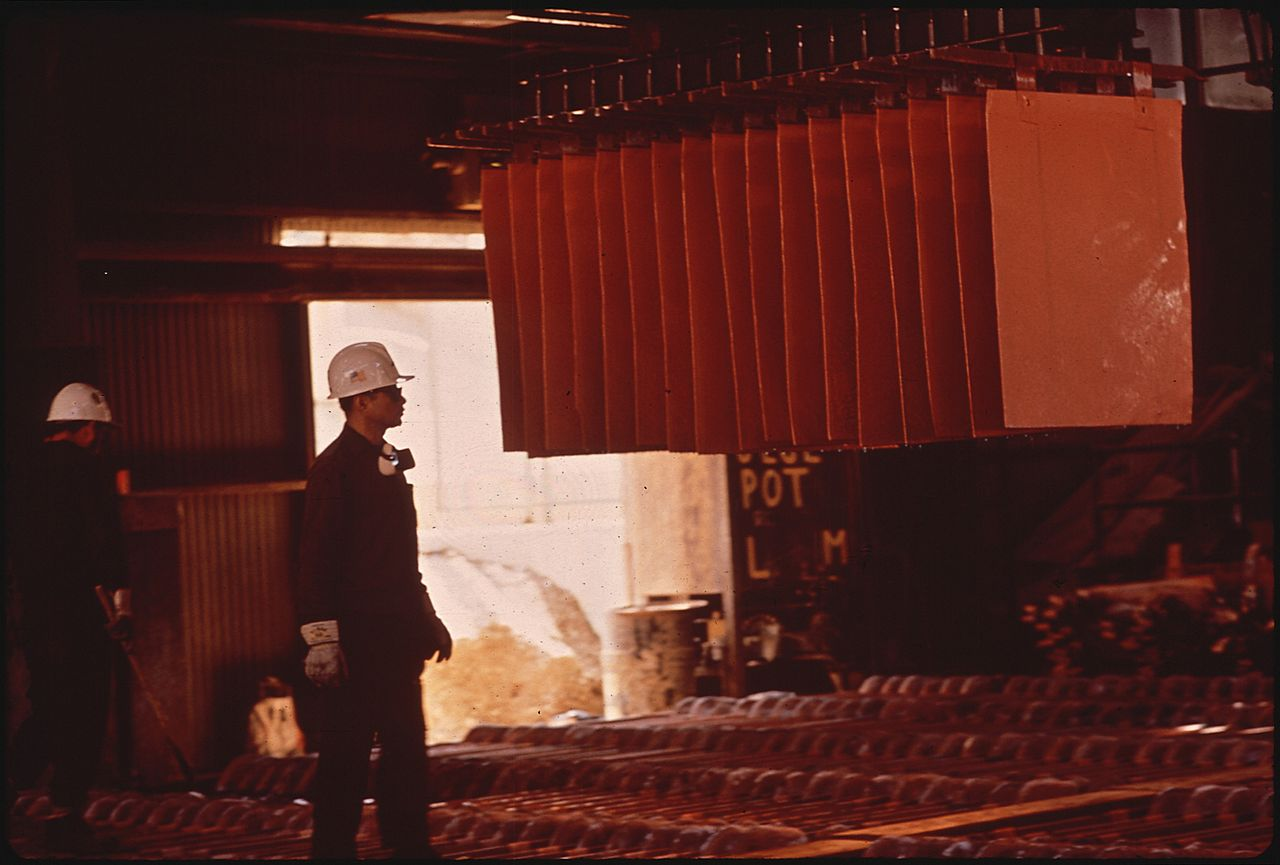
\includegraphics[width=.9\textwidth]{img/Copper-anodes.jpg}
		\caption*{Měděné anody.\footnote[frame]{\href{https://commons.wikimedia.org/wiki/File:ELECTROWINNING_REFINING_PLANT,_PART_OF_ARIZONA\%27S_EXTENSIVE_COPPER_INDUSTRY_-_NARA_-_544053.jpg}{Zdroj: U.S. National Archives and Records Administration/Commons}}}
	\end{figure}
	\vfill
}

\frame{
	\frametitle{}
	\vfill
	\begin{figure}
		\adjincludegraphics[height=.7\textheight]{img/Copper_Flash_Smelting_Process.png}
		\caption*{Schéma výroby mědi.\footnote[frame]{\href{https://commons.wikimedia.org/wiki/File:Copper_Flash_Smelting_Process_(EN).svg}{Zdroj: US Environmental Protection Agency/Commons}}}
	\end{figure}
	\vfill
}

\frame{
	\frametitle{}
	\vfill
	\begin{itemize}
		\item Až 80~\% mědi se získává recyklací.
		\item Měď je po železe a hliníku třetí kov, který se nejvíce recykluje.
		\item Během recyklace nedochází ke snížení kvality.
		\item Měděný šrot je roztaven a následně redukován.
		\item Poté se tavenina odlévá do ingotů.
		\item Znečištěný šrot je rafinován elektrolyticky.
	\end{itemize}
	\begin{figure}
		\adjincludegraphics[height=.5\textheight]{img/Copper-ingots.jpg}
	\end{figure}
	\vfill
}

\subsection{Stříbro}
\frame{
	\frametitle{}
	\vfill
	\textbf{Akantit}
	\begin{itemize}
		\item Jednoklonný sulfidický minerál, \ce{Ag2S},\footnote[frame]{\href{https://mineraly.sci.muni.cz/sulfidy/akantit.html}{Akantit}} šedé až černé barvy.\footnote[frame]{\href{https://www.mindat.org/min-10.html}{Acanthite}}
		\item Poprvé byl popsán v roce 1855 v Jáchymově.\footnote[frame]{\href{http://files.jachymov-joachimsthal.cz/200000225-a7397a833b/035\%20Akantit.pdf}{G. A. Kenngott}}
	\end{itemize}

	\begin{columns}
		\begin{column}{.5\textwidth}
			\begin{figure}
				\adjincludegraphics[height=.4\textheight]{img/Acanthite.jpg}
			\end{figure}
		\end{column}
		\begin{column}{.5\textwidth}
			\begin{figure}
				\adjincludegraphics[height=.4\textheight]{img/Acanthite-113670.jpg}
			\end{figure}
		\end{column}
	\end{columns}
	\vfill
}

\frame{
	\frametitle{}
	\vfill
	\textbf{Pyrargyrit}
	\begin{itemize}
		\item Trigonální sulfidický minerál, \ce{Ag3SbS3},\footnote[frame]{\href{https://mineraly.sci.muni.cz/sulfidy/pyrargyrit.html}{Pyrargyrit}} tmavě červené až šedé barvy.\footnote[frame]{\href{https://www.mindat.org/min-3313.html}{Pyrargyrite}}
		\item Důležitý zdroj stříbra.
	\end{itemize}

	\begin{columns}
		\begin{column}{.5\textwidth}
			\begin{figure}
				\adjincludegraphics[height=.4\textheight]{img/Pyrargyrite-177493.jpg}
			\end{figure}
		\end{column}
		\begin{column}{.5\textwidth}
			\begin{figure}
				\adjincludegraphics[height=.4\textheight]{img/Pyrargyrite.jpg}
			\end{figure}
		\end{column}
	\end{columns}
	\vfill
}

\frame{
	\frametitle{}
	\vfill
	\begin{itemize}
		\item Hlavními zdroji stříbra jsou rudy mědi, olova a zinku.
		\item Získává se jako vedlejší produkt výroby těchto kovů.\footnote[frame]{\href{https://www.youtube.com/watch?v=JFMyReR6HBY}{Jak se co dělá - Stříbro}}
		\item Anodové kaly z výroby mědi se zpracovávají horkou \ce{H2SO4} za současného vhánění vzduchu, čímž dojde k rozpuštění části kovů.
		\item Zbytek je zahříván s křemenem nebo vápnem, čímž přejde většina kovů do strusky.
		\item Stříbro se izoluje z dusičnanového roztoku elektrolyticky.
		\item Stejně jako v případě mědi je důležitým zdrojem i recyklace stříbra.\footnote[frame]{\href{https://blog.emew.com/silver-recovery-from-scrap-and-low-grade-residue}{Silver Recovery from Scrap and Low-Grade Residue}}
		\item Komerční stříbro má čistotu minimálně 99,9~\%.
	\end{itemize}
	\begin{figure}
		\adjincludegraphics[height=.35\textheight]{img/Silver.jpg}
	\end{figure}
	\vfill
}

\subsection{Zlato}
\frame{
	\frametitle{}
	\vfill
	\textbf{Krennerit}
	\begin{itemize}
		\item Orthorombický minerál, \ce{Au3AgTe8}, stříbrno-bílé barvy.\footnote[frame]{\href{https://www.mindat.org/min-2274.html}{Krennerite}}
		\item Jeho složení je závislé na lokalitě, limitní složení jsou \ce{AuTe2} a \ce{Au3AgTe8}.
	\end{itemize}

	\begin{columns}
		\begin{column}{.5\textwidth}
			\begin{figure}
				\adjincludegraphics[height=.4\textheight]{img/Krennerite-118303.jpg}
			\end{figure}
		\end{column}
		\begin{column}{.5\textwidth}
			\begin{figure}
				\adjincludegraphics[height=.4\textheight]{img/Krennerite-118304.jpg}
			\end{figure}
		\end{column}
	\end{columns}
	\vfill
}

\frame{
	\frametitle{}
	\vfill
	\textbf{Petzit}
	\begin{itemize}
		\item Kubický minerál, \ce{Ag3AuTe2}, šedé až černé barvy.\footnote[frame]{\href{https://www.mindat.org/min-3180.html}{Petzite}}
		\item Často se vyskytuje společně s dalšími minerály telluru a zlata.
	\end{itemize}

	\begin{columns}
		\begin{column}{.5\textwidth}
			\begin{figure}
				\adjincludegraphics[height=.4\textheight]{img/Petzite-784592.jpg}
			\end{figure}
		\end{column}
		\begin{column}{.5\textwidth}
			\begin{figure}
				\adjincludegraphics[height=.4\textheight]{img/Petzite-784598.jpg}
			\end{figure}
		\end{column}
	\end{columns}
	\vfill
}

\frame{
	\frametitle{}
	\vfill
	\begin{itemize}
		\item Zlato se dříve získávalo rýžováním říčních písků, ale tyto zdroje jsou již dnes vyčerpány.
	\end{itemize}

	\begin{columns}
		\begin{column}{.5\textwidth}
			\begin{figure}
				\adjincludegraphics[width=\textwidth]{img/Gold_Pan.jpg}
			\end{figure}
		\end{column}
		\begin{column}{.5\textwidth}
			\begin{figure}
				\adjincludegraphics[width=\textwidth]{img/Gold_in_the_pan.jpg}
			\end{figure}
		\end{column}
	\end{columns}
	\vfill
}

\frame{
	\frametitle{}
	\vfill
	\begin{itemize}
		\item Území dnešní ČR bylo a stále je bohaté na zlato.
		\item Těžba zlata zde probíhala už ve 3. století př. n. l.\footnote[frame]{\href{https://sever.rozhlas.cz/historie-tezby-zlata-u-nas-7794021}{Historie těžby zlata u nás}}
		\item Nejvíce zlata se vytěžilo ve 13. a 14. století za vlády Jana Lucemburského a Karla IV., kdy těžba probíhala prakticky na celém území.
		\item Nejdůležitější lokality jsou:
		\begin{itemize}
			\item Jílovský revír u Prahy
			\item Knínská zlatonosná oblast ve středním Povltaví
			\item Kašperské hory
			\item Pozůstatky povrchových dolů v okrese Klatovy (Hartmanice) jsou kulturní památkou České republiky.\footnote[frame]{\href{https://pamatkovykatalog.cz/povrchove-doly-na-zlato-14583576}{Povrchové doly na zlato}}
		\end{itemize}
		\item Podle odhadů bylo na našem území vytěženo 100 tun zlata, jak povrchovým, tak i hlubinným způsobem.
		\item Zhruba stejné množství zlata je stále uloženo v zemi.
	\end{itemize}
	\vfill
}

\frame{
	\frametitle{}
	\vfill
	\begin{figure}
		\adjincludegraphics[height=.7\textheight]{img/Hamizna.jpg}
		\caption*{Pozůstatky po dolování v lokalitě Hartmanice}
	\end{figure}
	\vfill
}

\frame{
	\frametitle{}
	\vfill
	\begin{itemize}
		\item Dnes se využívají hlavně horniny s dostatečným obsahem zlata.
		\item Pro ekonomické využití je nutná koncentrace alespoň 0,5 ppm.
		\item Hornina se rozemele na jemný prášek a zlato se pak získává buď tvorbou amalgámu a následným oddestilováním rtuti.
		\item To je ekologicky velmi nešetrný způsob.\footnote[frame]{\href{https://www.science.org/content/article/illegal-gold-mines-flood-amazon-forests-toxic-mercury}{Illegal gold mines flood Amazon forests with toxic mercury}}
		\item Druhý způsob je reakcí s alkalickým kyanidem a kyslíkem:
		\item \ce{4 Au + 8 NaCN + O2 + 2 H2O -> 4 Na[Au(CN)2] + 4 NaOH}
		\item Zlato lze pak izolovat reakcí se zinkovým prachem:
		\item \ce{2 Na[Au(CN)2] + Zn -> Na2[Zn(CN)4] + 2 Au}
		\item Zlato je poté odfiltrováno a přetaveno do podoby tyčí, které jsou dále rafinovány.
		\item Kyanidový způsob s sebou také nese riziko ekologických škod, v minulosti bylo zaznamenáno několik velkých havárií spojených s těžbou zlata.\footnote[frame]{\href{https://en.wikipedia.org/wiki/List_of_gold_mining_disasters}{List of gold mining disasters}}
	\end{itemize}
	\vfill
}

\frame{
	\frametitle{}
	\vfill
	\textbf{Největší producenti zlata v letech 2016 a 2017}\footnote[frame]{\href{https://s3-us-west-2.amazonaws.com/prd-wret/assets/palladium/production/mineral-pubs/mcs/mcs2018.pdf}{Mineral commodity summaries 2018}}
	\begin{center}
		\begin{tabular}{|l|l|l|}
		\hline
		\multicolumn{3}{|c|}{\textbf{Produkce zlata v tunách}}\\\hline
		\textbf{Země} & \textbf{2016} & \textbf{2017} \\\hline
		Čína & 453 & 440 \\\hline
		Austrálie & 290 & 300 \\\hline
		Rusko & 253 & 255 \\\hline
		USA & 222 & 245 \\\hline
		Kanada & 165 & 180 \\\hline
		Peru & 153 & 155 \\\hline
		Jižní Afrika & 145 & 145 \\\hline
		Mexiko & 111 & 110 \\\hline
		Uzbekistán & 102 & 100 \\\hline
		Brazílie & 85 & 85 \\\hline
		Indonésie & 80 & 80 \\\hline
	\end{tabular}
	\end{center}
	\vfill
}

\frame{
	\frametitle{}
	\vfill
	\begin{figure}
		\adjincludegraphics[width=\textwidth]{img/Map_of_gold_production.png}
	\end{figure}
	\vfill
}

\section{Využití}
\subsection{Měď}
\frame{
	\frametitle{}
	\vfill
	\begin{itemize}
		\item Měď je už dvě století využívána pro výrobu elektrických vodičů a kontaktů.
		\item Měrný elektrický odpor\footnote[frame]{Hodnota elektrického odporu 1 m vodiče} mědi je 16,78 n$\Omega$.m při teplotě 20~$^\circ$C.
		\item Zhruba 60~\% mědi se využívá na tyto aplikace.
		\item Vlivem velkých změn v energetické infrastruktuře silně roste poptávka po mědi a klesá její dostupnost.\footnote[frame]{\href{https://www.intellinews.com/the-copper-shortage-is-getting-real-265590/}{The copper shortage is getting real}}
	\end{itemize}
	\begin{columns}
		\begin{column}{.5\textwidth}
			\begin{tabular}{|l|r@{,}l|}
			\hline
			\textbf{Materiál} &
			\multicolumn{2}{c|}{\textbf{Měrný odpor [n$\Omega$.m]}} \\\hline
			Stříbro & 15 & 9 \\\hline
			Měď & 16 & 8 \\\hline
			Zlato & 24 & 4 \\\hline
			Hliník & 26 & 5 \\\hline
			Železo & 97 & 0 \\\hline
			Grafit & \multicolumn{2}{l|}{2500--5000} \\\hline
		\end{tabular}
		\end{column}
		\begin{column}{.5\textwidth}
			\begin{figure}
				\adjincludegraphics[width=\textwidth]{img/Tubo_di_rame.jpg}
			\end{figure}
		\end{column}
	\end{columns}
	\vfill
}

\frame{
	\frametitle{}
	\vfill
	\begin{itemize}
		\item V elektronice se dále využívá i velmi dobré tepelné vodivosti mědi.
		\item Měděné chladiče se používají k chlazení zesilovačů, výkonových součástek, CPU, $\ldots$
		\item Měďěné dráty se také využívají pro konstrukci vinutí cívek motorů.
	\end{itemize}

		\begin{columns}
		\begin{column}{.5\textwidth}
			\begin{figure}
				\adjincludegraphics[height=.4\textheight]{img/Heatsinkrods.jpg}
			\end{figure}
		\end{column}
		\begin{column}{.5\textwidth}
			\begin{figure}
				\adjincludegraphics[height=.4\textheight]{img/MakePCB-step6a.jpg}
			\end{figure}
		\end{column}
	\end{columns}
	\vfill
}

\frame{
	\frametitle{}
	\vfill
	\begin{itemize}
		\item Další velká oblast využití mědi (asi 20~\%) je stavebnictví. Zde se využívá korozní odolnosti a časové stability mědi.
		\item Měď po čase získává charakteristické zelené zabarvení způsobené oxidací -- vzniká hydroxid-síran nebo hydroxid-uhličitan měďnatý.
	\end{itemize}
	\begin{figure}
		\adjincludegraphics[height=.55\textheight]{img/Trencin-synagoga.jpg}
		\caption*{Synagoga v Trenčíně}
	\end{figure}
	\vfill
}

\frame{
	\frametitle{}
	\vfill
	\begin{columns}
		\begin{column}{.65\textwidth}
			\begin{itemize}
				\item \textbf{Dural} nebo \textbf{duraliminium} je skupina slitin hliníku s mědí, hořčíkem, manganem a dalšími kovy.
				\item Např. dural 3003 obsahuje 0,5~\% mědi, 1~\% manganu.\footnote[frame]{\href{https://unitedaluminum.com/aluminum-3003-alloy/}{Aluminum alloy 3003}}
				\item Slitina byla vyvinuta v roce 1909.
				\item Využívá se hlavně v automobilovém a leteckém průmyslu, ale také při výrobě sportovních a zdravotních pomůcek.
			\end{itemize}
		\end{column}
		\begin{column}{.35\textwidth}
			\begin{figure}
				\adjincludegraphics[width=\textwidth]{img/Akron_duralumin_sample.jpg}
				\caption*{Vzorek duralu použitého pro konstrukci vzducholodi USS Akron}
			\end{figure}
		\end{column}
	\end{columns}
	\vfill
}

\frame{
	\frametitle{}
	\vfill
	\begin{itemize}
		\item Měď a její slitiny mají baktericidní účinky.
		\item V roce 1852 zjistil Victor Burq, že zaměstnanci měďných hutí jsou výrazněji odolnější vůči epidemii cholery než jiní lidé.\footnote[frame]{\href{https://www.vice.com/en/article/xgqkyw/copper-destroys-viruses-and-bacteria-why-isnt-it-everywhere}{Copper Destroys Viruses and Bacteria. Why Isn’t It Everywhere?}}
		\item Čím je vyšší aktivní povrch mědi, tím jsou její antimikrobiální účinky vyšší.
		\item Velmi výrazného zrychlení a zvýšení účinnosti lze dosáhnout přípravou porézní mědi.\footnote[frame]{\href{https://www.osel.cz/12066-pozoruhodna-mikro-nanomed-zabiji-bakterie-skoro-jako-bajna-meduza.html}{Pozoruhodná mikro-nanoměď zabíjí bakterie skoro jako bájná Medúza}}
		\item Tu můžeme získat např. ze slitiny mědi a manganu selektivním odleptáním manganu.\footnote[frame]{\href{https://newatlas.com/materials/antibacterial-porous-copper/}{Special porous copper kills golden staph bacteria 120 times faster}}
	\end{itemize}
	\vfill
}

\subsection{Stříbro}
\frame{
	\frametitle{}
	\vfill
	\begin{columns}
		\begin{column}{.5\textwidth}
			\begin{itemize}
				\item Velká část stříbra se využívá ve šperkařství a výrobě mincí.
				\item Čisté stříbro nemá výhodné mechanické vlastnosti, proto se využívají slitiny s mědí.
				\item Nevýhodou stříbra je pomalé černání způsobené oxidací kyslíkem.
				\item Stříbrný vzhled lze obnovit pomocí hliníkové fólie, soli a vody, kdy dojde k elektrolytickému čištění.
			\end{itemize}
		\end{column}
		\begin{column}{.5\textwidth}
			\begin{figure}
				\adjincludegraphics[width=\textwidth]{img/Patzcuaro.jpg}
			\end{figure}
		\end{column}
	\end{columns}
	\vfill
}

\frame{
	\frametitle{}
	\vfill
	\begin{columns}
		\begin{column}{.5\textwidth}
			\begin{itemize}
				\item Světlocitlivosti solí stříbra se využívá v klasické fotografii.
				\item Na povrchu filmu je nanesena vrstva stříbrné soli s malým průměrem částic.
				\item Po dopadu světla dojde k černání filmu způsobeného vylučováním stříbra.
				\item V dnešní době trhu dominuje digitální fotografie, proto spotřeba stříbra v této oblasti klesá.\footnote[frame]{\href{https://www.bullionvault.com/gold-news/silver-bullion-photographic-demand-062120133}{A Big Source of Silver Bullion Demand Has Disappeared}}
			\end{itemize}
		\end{column}
		\begin{column}{.5\textwidth}
			\begin{figure}
				\adjincludegraphics[width=\textwidth]{img/Cinestill.jpg}
			\end{figure}
		\end{column}
	\end{columns}
	\vfill
}

\frame{
	\frametitle{}
	\vfill
	\begin{columns}
		\begin{column}{.7\textwidth}
			\begin{itemize}
				\item Rozprašováním malých částic jodidu stříbrného lze docílit tvorby mraků a~následného deště.
				\item Metoda je založena na tvorbě nukleačních center, jodid stříbrný ma podobnou krystalickou strukturu jako led.\footnote[frame]{\href{https://www.sacbee.com/news/local/article2582373.html}{Cloud seeding, no longer magical thinking, is poised for use this winter}}
				\item Rozprašování se provádí letadly.\footnote[frame]{\href{https://youtu.be/8GQAXxmiSdk}{Cloud seeding: How the UAE gets creative to increase rainfall}}
				\item Je to jedna z možností, jak zvýšit množství srážek v suchých oblastech.
			\end{itemize}
		\end{column}
		\begin{column}{.3\textwidth}
			\begin{figure}
				\adjincludegraphics[width=\textwidth]{img/Cloudseedingimagecorrected.jpg}
			\end{figure}
		\end{column}
	\end{columns}
	\vfill
}

\frame{
	\frametitle{}
	\vfill
	\begin{columns}
		\begin{column}{.6\textwidth}
			\textbf{Koloidní stříbro}
			\begin{itemize}
				\item Koloidní disperze stříbra ve vodě se využívají jako přípravky s baktericidními účinky.
				\item Aktivní sloužkou jsou ionty \ce{Ag+}, které narušují metabolismus bakterií.
				\item Nanočástice Ag se na vzduchu oxidují na \ce{Ag2O}, který ve vodném roztoku vytváří nízkou koncentraci \ce{Ag+}.
				\item Ta je dostatečná, aby se projevily baktericidní účinky.
			\end{itemize}
		\end{column}
		\begin{column}{.4\textwidth}
			\begin{figure}
				\adjincludegraphics[height=.7\textheight]{img/Plata_Coloidal_Super_Tyndall_Effect.jpg}
				\caption*{Koloidní stříbro.\footnote[frame]{\href{https://commons.wikimedia.org/wiki/File:Plata_Coloidal_Super_Tyndall_Effect.jpeg}{Zdroj: Silverliving/Commons}}}
			\end{figure}
		\end{column}
	\end{columns}
	\vfill
}

\subsection{Zlato}
\frame{
	\frametitle{}
	\vfill
	\begin{columns}
		\begin{column}{.4\textwidth}
			\begin{itemize}
				\item Hlavní využití zlata je v ekonomice a šperkařství.
				\item \textit{Zlatý standard} byl dříve využívám ke krytí měny hodnotou zlata v majetku emitenta.\footnote[frame]{\href{https://www.cnb.cz/cs/casto-kladene-dotazy/Cim-je-kryta-mena/}{Čím je kryta měna?}}
				\item Mince byly buď raženy ze zlata nebo jako platidlo sloužily bankovky, které byly kryté hodnotou zlata.
			\end{itemize}
		\end{column}
		\begin{column}{.5\textwidth}
			\begin{figure}
				\adjincludegraphics[width=\textwidth]{img/1_oz_of_Gold.jpg}
				\adjincludegraphics[width=\textwidth]{img/Czechoslovakia_1934_10_Ducats.jpg}
			\end{figure}
		\end{column}
	\end{columns}
	\vfill
}

\frame{
	\frametitle{}
	\vfill
	\begin{itemize}
		\item Čistota zlata se v klenotnictví udává v karátech (kt).\footnote[frame]{\href{https://www.sperky.cz/magazin/co-nam-rika-punc/}{Co nám říká punc?}}
		\item Čisté zlato ma \textit{ryzost} 24 kt.
		\item Ryzost je dána vztahem: $X = \frac{m_{Au}}{m}$.
	\end{itemize}

	\begin{tabular}{|l|l|l|l|l|l|l|l|}
		\hline
		\textbf{Karáty} & 9 & 14 & 18 & 21,6 & 22 & 23,6 & 24 \\\hline
		\textbf{Ryzostní číslo} & 5 & 4 & 3 & 2 & 1 & 0 & 00 \\\hline
	\end{tabular}

	\begin{figure}
		\adjincludegraphics[width=.85\textwidth]{img/Gold_necklace.jpg}
	\end{figure}
	\vfill
}

\frame{
	\frametitle{}
	\vfill
	\begin{itemize}
		\item V roce 2000 se spotřebovalo 280 tun zlata v elektronických aplikacích, spotřeba v této oblasti neustále roste.\footnote[frame]{\href{https://doi.org/10.1007/BF03214833}{Current and future uses of gold in electronics}}
		\item Hlavní využití zlata je pokovování konektorů, tím se sníží jejich odpor a zvýší odolnost vůči korozi.
		\item Dále se používá jako vodič v integrovaných obvodech a CPU.
	\end{itemize}

	\begin{columns}
		\begin{column}{.3\textwidth}
			\begin{figure}
				\adjincludegraphics[height=.4\textheight]{img/AMD-Duron.jpg}
			\end{figure}
		\end{column}
		\begin{column}{.7\textwidth}
			\begin{figure}
				\adjincludegraphics[height=.4\textheight]{img/Gold-plated_electrical_connectors.jpg}
			\end{figure}
		\end{column}
	\end{columns}
	\vfill
}

\frame{
	\frametitle{}
	\vfill
	\begin{itemize}
		\item Zlato má velmi dobrou odrazivost v oblasti viditelného i infračerveného záření, toho se využívá v optických aplikacích.
	\end{itemize}

	\begin{columns}
	\begin{column}{.3\textwidth}
		\begin{figure}
			\adjincludegraphics[height=.55\textheight]{img/Mirror_of_Hapiankhtifi.jpg}
		\end{figure}
	\end{column}
	\begin{column}{.7\textwidth}
		\begin{figure}
			\adjincludegraphics[height=.55\textheight]{img/GoldMirrors.jpg}
		\end{figure}
	\end{column}
	\end{columns}
	\vfill
}

\frame{
	\frametitle{}
	\vfill
	\begin{figure}
		\adjincludegraphics[height=.8\textheight]{img/TGIR1.jpg}
	\end{figure}
	\vfill
}

\frame{
	\frametitle{}
	\vfill
	\begin{itemize}
		\item Vesmírný dalekohled Jamese Webba je nástupce Hubbleova teleskopu.\footnote[frame]{\href{https://kosmonautix.cz/stitek/jwst/}{JWST na kosmonautix.cz}}
		\item Je umístěn v libračním centru L2 soustavy Země--Slunce, přibližně 1,5 milionu km od Země.
		\item Na rozdíl od Hubbleova teleskopu teleskop pracuje v oblasti infračerveného záření (0,6--28~$\mu$m).
		\item Aby bylo možné pracovat v IR oblasti je nutné, aby zrcadlo teleskopu bylo chlazené na velmi nízkou teplotu, pod 50~K.
		\item Zrcadla jsou vyrobena z beryllia, které je dostatečně lehké a mechanicky odolné. Velkou výhodou je i jeho nízká tepelná roztažnost.
		\item Celková plocha zrcadla je 25~m$^2$ a je potaženo vrstvou zlata o tloušťce přibližně 100~nm.\footnote[frame]{\href{https://webb.nasa.gov/content/observatory/ote/mirrors/index.html}{Mirrors Webb/NASA}}
		\item Teleskop odstartoval 25. prosince 2021 na raketě Ariane 5, do bodu L2 dorazil přibližně za měsíc od startu.
		\item V současnosti je už téměř připraven k ostrému provozu.
	\end{itemize}
	\vfill
}

\frame{
	\frametitle{}
	\vfill
	\begin{figure}
		\adjincludegraphics[height=.82\textheight]{img/Lagrange_points.jpg}
	\end{figure}
	\vfill
}

\frame{
	\frametitle{}
	\vfill
	\begin{columns}
		\begin{column}{.65\textwidth}
			\begin{figure}
				\adjincludegraphics[width=\textwidth]{img/JWST-HST-primary-mirrors.png}
			\end{figure}
		\end{column}
		\begin{column}{.4\textwidth}
			\begin{figure}
				\adjincludegraphics[width=\textwidth]{img/Ariane_5_Le_Bourget_FRA_001.jpg}
			\end{figure}
		\end{column}
	\end{columns}
	\vfill
}

\frame{
	\frametitle{}
	\vfill
	\begin{columns}
		\begin{column}{.5\textwidth}
		\begin{figure}
		\adjincludegraphics[height=.7\textheight]{img/JWST_Mirrors.jpg}
		\end{figure}
		\end{column}
		\begin{column}{.5\textwidth}
			\begin{figure}
				\adjincludegraphics[height=.6\textheight]{img/James_Webb_Space_Telescope_Artist_Conception.jpg}
			\end{figure}
		\end{column}
	\end{columns}
	\begin{center}
		Zrcadlo \href{https://www.stsci.edu/jwst/}{vesmírného dalekohledu Jamese Webba}.
	\end{center}
	\vfill
}

\frame{
	\frametitle{}
	\vfill
	\begin{figure}
		\adjincludegraphics[height=.82\textheight]{img/JWST_Telescope_alignment_evaluation_image_labeled.jpg}
	\end{figure}
	\vfill
}

\frame{
	\frametitle{}
	\vfill
	\textbf{Jedlé zlato}
	\begin{columns}
		\begin{column}{.6\textwidth}
			\begin{itemize}
				\item Potravinářské aditivum E175,\footnote[frame]{\href{https://www.ferpotravina.cz/seznam-ecek/E175}{E175 - Zlato}} jeho čistota musí být 23--24 karátů, aby byla vyloučena přítomnost toxických kovů.\footnote[frame]{\href{https://www.stoplusjednicka.cz/vzacny-kov-na-taliri-je-mozne-bez-zdravotnich-nasledku-snist-zlato}{Vzácný kov na talíři: Je možné bez zdravotních následků sníst zlato?}}
				\item Vzhledem k nízké reaktivitě zlata, dokáže projít trávícím traktem, aniž by došlo ke vzniku zdravotního rizika.\footnote[frame]{\href{https://youtu.be/E0snFza8Xqo}{Is A \$90 24-Karat Gold Burger Worth It?}}
				\item Konzumace zlata se datuje až do starověkého Egypta.
			\end{itemize}
		\end{column}
		\begin{column}{.4\textwidth}
			\begin{figure}
				\adjincludegraphics[width=\textwidth]{img/Golden_cake.jpg}
			\end{figure}
		\end{column}
	\end{columns}
	\vfill
}

\section{Sloučeniny}
\subsection{Měď}
\frame{
	\frametitle{}
	\vfill
	\begin{itemize}
		\item Měď vytváří sloučeniny v rozmezí oxidačních čísel 0 až +IV. Nejběžnější jsou I a II.
		\item Karbonylové sloučeniny v oxidačním číslo \ce{Cu^0} jsou stabilní jen za kryogenních podmínek.
	\end{itemize}
	\begin{center}
	\begin{tabular}{|l|l|}
		\hline
		\textbf{Ox. číslo} & \textbf{Sloučenina} \\\hline
		0 & \ce{Cu(CO)3} \\\hline
		1 & \ce{Cu2O}, \ce{[CuCl2]-} \\\hline
		2 & \ce{CuSO4.5H2O}, \ce{Cs2[CuCl4]} \\\hline
		3 & \ce{[CuF6]^{3-}} \\\hline
		4 & \ce{[CuF6]^{2-}} \\\hline
	\end{tabular}
	\end{center}
	\vfill
}

\frame{
	\frametitle{}
	\vfill
	\begin{itemize}
		\item Modrá skalice, pentahydrát síranu měďnatého, je modrá pevná látka se vzorcem \ce{CuSO4.5H2O}.
		\item Ve vodném roztoku vytváří oktaedrický komplex, \ce{[Cu(H2O)6]^{2+}}.
		\item Používá se jako herbicid a fungicid.
	\end{itemize}

	\begin{columns}
	\begin{column}{.5\textwidth}
		\begin{figure}
			\adjincludegraphics[height=.4\textheight]{img/Copper_Sulfate_Crystal.jpg}
			\caption*{Modrá skalice}
		\end{figure}
	\end{column}
	\begin{column}{.5\textwidth}
		\begin{figure}
			\adjincludegraphics[height=.4\textheight]{img/Copper_sulfate_anhydrous.jpg}
			\caption*{Bezvodý síran měďnatý}
		\end{figure}
	\end{column}
\end{columns}

	\vfill
}

\frame{
	\frametitle{}
	\vfill
	\begin{figure}
		\adjincludegraphics[height=1.2\textheight,rotate=270]{img/CuSO4-TG.png}
		\caption*{Termogravimetrická analýza modré skalice}
	\end{figure}
	\vfill
}

\frame{
	\frametitle{}
	\vfill
	\begin{itemize}
		\item Vzhledem k elektrodovému potenciálu mědi (+0,34~V), nemůže měď reagovat s kyselinou sírovou za vzniku vodíku.
		\item Kyselina sírová nejprve oxiduje měď:
		\item \ce{Cu + H2SO4 ->[T] CuO + SO2 + H2O}
		\item Vzniklý oxid pak reaguje s další kyselinou sírovou za vzniku síranu:
		\item \ce{CuO + H2SO4 -> CuSO4 + H2O}
		\item Celková reakce je tedy:
		\item \ce{Cu + 2 H2SO4 ->[T] CuSO4 + SO2 + 2 H2O}
		\item Alternativní možností je využít k oxidaci kyselinu dusičnou:
		\item \ce{3 Cu + 2 HNO3 -> 3 CuO + H2O + 2 NO}
		\item \ce{CuO + H2SO4 -> CuSO4 + H2O}
	\end{itemize}
	\vfill
}

\frame{
	\frametitle{}
	\vfill
	\begin{itemize}
		\item První organokovovou sloučeninou mědi byl červený acetylid měďný, připravený v roce 1859 reakcí:
		\item \ce{2 CuCl + C2H2 ->[NH3] Cu2C2 + 2 HCl}
		\item Tato sloučenina je velmi citlivá na náraz a změny teploty, snadno exploduje.
		\item Reakce halogenidů měďných s organolithnými sloučeninami poskytují organoměďné látky:
		\item \ce{CuCl + 2 MeLi -> Me2CuLi + LiCl}
		\item \ce{CuMe + MeLi -> Me2CuLi}
		\item Tyto sloučeniny se označují jako Gilmanovy reagenty, reakcí s organohalogenidem vytváří vazbu \ce{C-C}.\footnote[frame]{\href{https://dx.doi.org/10.1055/s-1972-21833}{Organocopper(I) Compounds and Organocuprates in Synthesis}}
		\item \ce{Me2CuLi + EtCl -> Me-Cu + \textbf{Me-Et} + LiCl}
	\end{itemize}
	\vfill
}

\subsection{Stříbro}
\frame{
	\frametitle{}
	\vfill
	\begin{itemize}
		\item Stříbro vytváří sloučeniny v rozmezí oxidačních čísel 0 až +III. Nejběžnější oxidační číslo je I.
		\item Karbonylové sloučeniny v oxidačním číslo \ce{Ag^0} jsou stabilní jen za kryogenních podmínek.
	\end{itemize}
	\begin{center}
		\begin{tabular}{|l|l|}
			\hline
			\textbf{Ox. číslo} & \textbf{Sloučenina} \\\hline
			0 & \ce{Ag(CO)3} \\\hline
			1 & \ce{AgCl} \\\hline
			2 & \ce{[Ag(py)4]^{2+}}, \ce{AgF2} \\\hline
			3 & \ce{AgF3}, \ce{[AgF4]^{-}}, \ce{[AgF6]^{3-}} \\\hline
		\end{tabular}
	\end{center}
	\vfill
}

\frame{
	\frametitle{}
	\vfill
	\begin{itemize}
		\item Všechny halogenidy stříbrné jsou \textit{fotocitlivé}.
		\item Fluorid stříbrný, \ce{AgF}, je žluto-hnědá pevná látka. Na rozdíl od ostatních halogenidů stříbrných je rozpustný ve vodě.
		\item Můžeme jej připravit reakcí uhličitanu nebo oxidu stříbrného s fluorovodíkem:\footnote[frame]{\href{https://dx.doi.org/10.3891/acta.chem.scand.07-0236}{Laboratory Preparation of the Fluorinating Agents \ce{SbF3} and AgF}}
		\item \ce{Ag2CO3 + 2 HF -> 2 AgF + H2O + CO2}
		\item Chlorid stříbrný, AgCl, je bílá pevná látka. Je nerozpustný ve vodě, čehož se využívá v \textit{argentometrii}.
		\item V přírodě se vyskytuje jako minerál \textit{chlorargyrit}.\footnote[frame]{\href{https://www.mindat.org/min-1014.html}{Chlorargyrite}}
		\item Bromid stříbrný, AgBr, je nažloutlá pevná látka, nerozpustná ve vodě.
		\item Jodid stříbrný, AgI, je žlutá pevná látka, nerozpustná ve vodě.
	\end{itemize}
	\vfill
}

\frame{
	\frametitle{}
	\vfill
	\begin{figure}
		\adjincludegraphics[height=.75\textheight]{img/Common_Silver_Halide_Precipitates.jpg}
		\caption*{Jodid, bromid a chlorid stříbrný}
	\end{figure}
	\vfill
}

\frame{
	\frametitle{}
	\vfill
	\begin{columns}
		\begin{column}{.7\textwidth}
			\begin{itemize}
		\item \textbf{Argentometrie}
		\item Metoda srážecí odměrné analýzy.
		\item Jako odměrný roztok se využívá \ce{AgNO3}.
		\item Hlavní využití je ke stanovení chloridů, např.v  pitné vodě:
		\item \ce{AgNO3 + KCl -> AgCl v + KNO3}
		\item Indikátorem je chroman draselný:
		\item \ce{2 AgNO3 + K2CrO4 -> Ag2CrO4 v + 2 KNO3}
		\item Argentometricky lze stanovit všechny halogenidy, kromě fluoridů.
	\end{itemize}
	\begin{tabular}{|l|l|l|l|}
	\hline
	\textbf{Halogenid} & AgCl & AgBr & AgI \\\hline
	p$K_s$ & 9,80 & 12,20 & 15,82 \\\hline
	\end{tabular}
	\end{column}
	\begin{column}{.3\textwidth}
		\begin{figure}
			\adjincludegraphics[width=\textwidth]{img/Argentometry.jpg}
		\end{figure}
	\end{column}
	\end{columns}
	\vfill
}

\frame{
	\frametitle{}
	\vfill
	\begin{itemize}
		\item \textbf{Gravimetrické stanovení chloridů ve formě AgCl}
		\item Chloridy se sráží za chladu roztokem dusičnanu stříbrného v prostředí \ce{HNO3}.
		\item Po kvantitativním vysrážením se roztok zahřeje téměř k varu.
		\item Poté se nechá dvě hodiny stát v temnu, aby nedocházelo k rozkladu světlem.
		\item Po filtraci se promývá, až do negativní reakce na stříbrné ionty.
		\item Sraženina se následně suší při teplotě 130~$^\circ$C do konstantní hmotnosti.
	\end{itemize}
	\vfill
}

\frame{
	\frametitle{}
	\vfill
	\begin{itemize}
		\item Fluorid stříbrnatý, \ce{AgF2}, je jednou z mála sloučenin stříbra v oxidačním stavu II.
		\item Je to bílý krystalický prášek, postupně tmavne vznikajícími nečistotami.
		\item Lze ho připravit oxidací \ce{Ag2O} pomocí plynného fluoru nebo fluoridu, příp. chloridu stříbrného za vyšší teploty:
		\item \ce{2 Ag2O + 2 F2 -> 2 AgF2 + O2}
		\item \ce{2 AgF + F2 ->[200 $^\circ$C] 2 AgF2}
		\item Neutronovou difrakcí bylo prokázáno, že se jedná skutečně o \ce{AgF2} a ne o komplexní fluorid (\ce{Ag^I[Ag^{III}F4]}).\footnote[frame]{\href{https://doi.org/10.1021/ja051442j}{Structure and Bonding in Silver Halides. A Quantum Chemical Study $\ldots$}}
		\item Využívá se jako velmi silné oxidační a fluorační činidlo, dokáže fluorovat benzen, i plynný xenon:
		\item \ce{C6H6 + 2 AgF2 -> C6H5F + 2 AgF + HF}\footnote[frame]{\href{https://doi.org/10.1021/jo01306a011}{New method for selective monofluorination of aromatics using silver difluoride}}
		\item \ce{Xe + 2 AgF2 ->[HF] XeF2 + 2 AgF}\footnote[frame]{\href{https://doi.org/10.1016/0022-1902(74)80203-4}{On the reaction between xenon and fluorine}}
	\end{itemize}
	\vfill
}

\frame{
	\frametitle{}
	\vfill
	\begin{figure}
		\adjincludegraphics[height=.75\textheight]{img/Ag2F-3D-ionic.png}
		\caption*{Krystalová struktura \ce{AgF2}. Zdroj: \href{https://commons.wikimedia.org/wiki/File:Silver(II)-fluoride-3D-ionic.png}{Benjah-bmm27/Commons}}
	\end{figure}
	\vfill
}

\frame{
	\frametitle{}
	\vfill
	\begin{itemize}
		\item Fluorid stříbrnitý, \ce{AgF3}, je nestabilní fluorid, ve kterém má stříbro oxidační stav III.
		\item Je to červená, diamagnetická látka, má podobnou krystalovou strukturu jako fluorid zlatitý.\footnote[frame]{\href{https://doi.org/10.1021/ja00011a021}{Silver trifluoride: preparation, crystal structure, some properties, and comparison with \ce{AuF3}}}
		\item Připravuje se reakcí draslíku s dusičnanem stříbrným a fluorem za zvýšeného tlaku a teploty:\footnote[frame]{\href{https://doi.org/10.2172/7017272}{The synthesis and structural characterization of novel transition metal fluorides}}
		\item \ce{2 K + AgNO + 2 F2 ->[400 $^\circ$C] K[AgF4] + KNO3}
		\item a následnou reakcí s \ce{BF3}:
		\item \ce{K[AgF4] + BF3 -> AgF3 + K[BF4]}
	\end{itemize}
	\vfill
}

\subsection{Zlato}
\frame{
	\frametitle{}
	\vfill
	\begin{itemize}
		\item Zlato vytváří sloučeniny v rozmezí oxidačních čísel $-$I až +V. Nejběžnější oxidační stavy jsou I a III.
		\item V kapalném amoniaku vytváří komplexní ion \ce{[Au(NH3)_n]-}.
		\item Reakcí AuF s \ce{HF/SbF5} v přítomnosti xenonu vzniká sloučenina \ce{(AuXe4)(Sb2F11)2}, obsahuje planární kation \ce{AuXe4}.\footnote[frame]{\href{https://doi.org/10.1126/science.290.5489.117}{Xenon as a Complex Ligand: The Tetra Xenono Gold(II) Cation}}
	\end{itemize}
	\begin{center}
		\begin{tabular}{|l|l|}
			\hline
			\textbf{Ox. číslo} & \textbf{Sloučenina} \\\hline
			$-$1 & \ce{[Au(NH3)_n]-}, \ce{CsAu} \\\hline
			1 & \ce{[Au(CN)2]-} \\\hline
			2 & \ce{[Au\{S2C2(CN)2\}2]^{2-}} \\\hline
			3 & \ce{AuF3}, \ce{Au2Cl6}, \ce{[AuBr4]-} \\\hline
			5 & \ce{[AuF6]^{-}} \\\hline
		\end{tabular}
	\end{center}
	\vfill
}

\frame{
	\frametitle{}
	\vfill
	\begin{columns}
		\begin{column}{.75\textwidth}
			\begin{itemize}
				\item Fluorid zlatitý, \ce{AuF3}, je oranžová pevná látka, sublimuje při teplotě 300~$^\circ$C.
				\item Připravuje se fluorací chloridu zlatitého:
				\item \ce{2 AuCl3 + 3 F2 -> 2 AuF3 + 3 Cl2}
				\item Využívá se jako silné fluorační činidlo.\footnote[frame]{GREENWOOD, N. N. a Alan EARNSHAW. \textit{Chemie prvků.} Praha: Informatorium, 1993. ISBN 80-854-2738-9. s. 1467}
				\item Krystalová struktura se skládá ze čtvercových jednotek \ce{AuF4}, které jsou propojeny vrcholy do šroubovice.\footnote[frame]{\href{https://doi.org/10.1039/J19670000478}{The crystal structure of gold trifluoride}}
			\end{itemize}
		\end{column}
		\begin{column}{.2\textwidth}
			\begin{figure}
				\adjincludegraphics[width=\textwidth]{img/Gold-trifluoride-spiral-side-3D-balls.png}
			\end{figure}
		\end{column}
	\end{columns}
	\vfill
}

\frame{
	\frametitle{}
	\vfill
	\begin{columns}
		\begin{column}{.5\textwidth}
			\begin{itemize}
				\item Zlatid cesný, CsAu, je sůl obsahující cesný kation a zlatidový anion (\ce{Cs+Au-}).\footnote[frame]{\href{https://doi.org/10.1002/zaac.19613100304}{Das Verhalten der Alkalimetalle zu Kupfer, Silber und Gold}}
				\item Získává se zahříváním směsi cesia se zlatem.
				\item Hydrolýzou poskytuje hydroxid cesný a kovové zlato.
				\item \ce{2 CsAu + 2 H2O -> 2 CsOH + 2 Au + 2 H2}
			\end{itemize}
		\end{column}
		\begin{column}{.5\textwidth}
			\begin{figure}
				\adjincludegraphics[width=\textwidth]{img/CsCl_polyhedra.png}
			\end{figure}
		\end{column}
	\end{columns}
	\vfill
}

\frame{
	\frametitle{}
	\vfill
	\begin{columns}
		\begin{column}{.6\textwidth}
			\begin{itemize}
				\item V roce 2000 byla připravena první sloučenina vzácného plynu s ušlechtilým kovem.
				\item Reakcí fluoridu zlatitého s plynným xenonem v prostředí \ce{HF/SbF5} byla připravena sůl \ce{[AuXe4][Sb2F11]2}.
				\item Produkt se povedlo vykrystalovat ve dvou modifikacích -- v trojklonné a čtverečné soustavě.\footnote[frame]{\href{https://doi.org/10.1126/science.290.5489.117}{Xenon as a Complex Ligand: The Tetraxenonogold(II) Cation in \ce{AuXe$_4^{2+}$(Sb2F$_{11}^-$)2}}} Délka vazby \ce{Au-Xe} je 274~pm.
				\item Zlato má v této sloučenině oxidační číslo II.
			\end{itemize}
		\end{column}
		\begin{column}{.5\textwidth}
			\begin{figure}
				\adjincludegraphics[width=.9\textwidth]{img/AuXe4.png}
			\end{figure}
		\end{column}
	\end{columns}
	\begin{center}
		\ce{AuF3 + 6 Xe + 3 H+ ->[HF/SbF5] AuXe$_4^{2+}$ + Xe$_2^+$ + 3 HF}
	\end{center}
	\vfill
}

\frame{
	\frametitle{}
	\vfill
	\begin{columns}
		\begin{column}{.6\textwidth}
			\begin{itemize}
				\item Laserovou ablací kovového zlata v atmosféře plynného xenonu lze získat ionty obsahující vazbu \ce{Xe-Au}.\footnote[frame]{\href{https://doi.org/10.1039/D2CC05606B}{Spectroscopic evidence of a Xe–Xe bond in the linear \ce{Xe2Au+Xe} ion}}
				\item Hmotnostní spektrometrií bylo určeno složení iontů jako \ce{AuXe$_3^+$}.
				\item Tomuto složení odpovídají dva izomery.
				\item Pomocí infračervené spektroskopie bylo prokázáno, že vzniká lineární izomer, takže dochází i ke vzniku vazby \ce{Xe-Xe}.
			\end{itemize}
		\end{column}
		\begin{column}{.5\textwidth}
			\begin{figure}
				\adjincludegraphics[width=.9\textwidth]{img/Au-Xe.png}
			\end{figure}
		\end{column}
	\end{columns}
	\vfill
}

\section{Biologie}
\frame{
	\frametitle{}
	\vfill
	\begin{itemize}
		\item Měď patří mezi prvků důležité pro živé organismy.
		\item Vyskytuje se v řadě enzymatických cyklů, např. v metabolismu sachardidů a také při tvorbě kostní hmoty a červených krvinek.
		\item Měď je součástí \textit{hemocynianu}, analogu hemoglobinu u některých živočichů.
		\item Denní dávka mědi by se měla pohybovat mezi 1 a 100~mg. Zdroji mědi jsou ořechy, houby, korýši, měkkýši, játra a kakao.
		\item Nedostatek mědi se projevuje chudokrevností, zhoršením metabolismu sacharidů a zpomalením duševního vývoje.
		\item Při předávkování mědí hrozí podobné obtíže jako u kadmia a rtuti.
	\end{itemize}
	\vfill
}

\frame{
	\frametitle{}
	\vfill
	\begin{columns}
		\begin{column}{.6\textwidth}
			\begin{itemize}
				\item Hemocyanin, je metaloprotein obsahující dva ionty mědi.
				\item Je součástí respiračního cyklu měkkýšů a některých členovců.
				\item Ionty mědi slouží k navázání molekuly kyslíku.
				\item Při oxidaci přechází bezbarvá forma (\ce{Cu^I}) na modrou (\ce{Cu^I^I}).
			\end{itemize}

			\begin{figure}
				\adjincludegraphics[height=.3\textheight]{img/Oxyhemocyanin.png}
			\end{figure}
		\end{column}
		\begin{column}{.4\textwidth}
			\begin{figure}
				\adjincludegraphics[width=\textwidth]{img/Hemocyanin2.jpg}
			\end{figure}
		\end{column}
	\end{columns}
	\vfill
}

\input{../Last}

\end{document}